\documentclass{article}
\usepackage[a4paper, margin=5em]{geometry}
\usepackage{fancyhdr}
\usepackage{lastpage}
\usepackage{graphicx}
\usepackage{hyperref}
\usepackage{ngerman}
\usepackage{enumitem}
\usepackage{csquotes}

\newcommand{\gqq}[1]{\glqq{}#1\grqq{}}

\pagestyle{fancy}
\fancyhf{}
\renewcommand{\headrulewidth}{0pt}
\fancyfoot{}

\lfoot{}
\cfoot{Seite \thepage\ / \pageref*{LastPage}}
\rfoot{}

\hypersetup{
    colorlinks=true,
    linktoc=all,
    linkcolor=blue
}

\author{Tim Wende}
\date{\today}
\title{\textbf{Übung 4}}

\begin{document}
    \maketitle

    \newpage
    \section{Aktivitätsdiagramm Fahrkartenautomat}
    In \href{https://www.ili.fh-aachen.de/ilias.php?ref_id=813760&obj_id=206096&obj_type=PageObject&cmd=layout&cmdClass=illmpresentationgui&cmdNode=gh&baseClass=ilLMPresentationGUI}{Übung 3} wurde ein Lastenheft für einen Fahrkartenautomaten erstellt.\\
    \begin{enumerate}[label=\alph*.]
        \item Dokumentieren Sie den Anwendungsfall \gqq{Fahrkarte kaufen} mit Hilfe eines \textbf{UML-Aktivitätsdiagrammmes}, das z.B. mit \href{https://www.ili.fh-aachen.de/ilias.php?baseClass=ilLinkResourceHandlerGUI&ref_id=341847&cmd=calldirectlink}{Visual Paradigm} erstellt wird.

            Teilen Sie das Aktivitätsdiagramm dabei in die folgenden Partitionen (Schwimmbahnen) auf:
            \begin{itemize}[label=◦]
                \item Kunde: Interaktion des Kunden mit dem Automaten
                \item Display: Anzeige von Text
                \item Automat: Eingaben einlesen, Rückgeldberechnung, Kartendruck, \ldots
            \end{itemize}
            
            Modellieren Sie dabei Geld und Fahrkarten als \textbf{Objektknoten}!
            
            Hinweise:
            \begin{itemize}[label=◦]
                \item Der Automat arbeitet nur mit Bargeld.
                \item Beachten Sie, dass der Bezahlvorgang auch abgebrochen werden kann.
                \item Verwenden Sie Parallelitäten, wo es für Sie Sinn ergibt.
                \item Beachten Sie auch den Fall, wenn der Automat nicht genug Rückgeld geben kann.
            \end{itemize}

            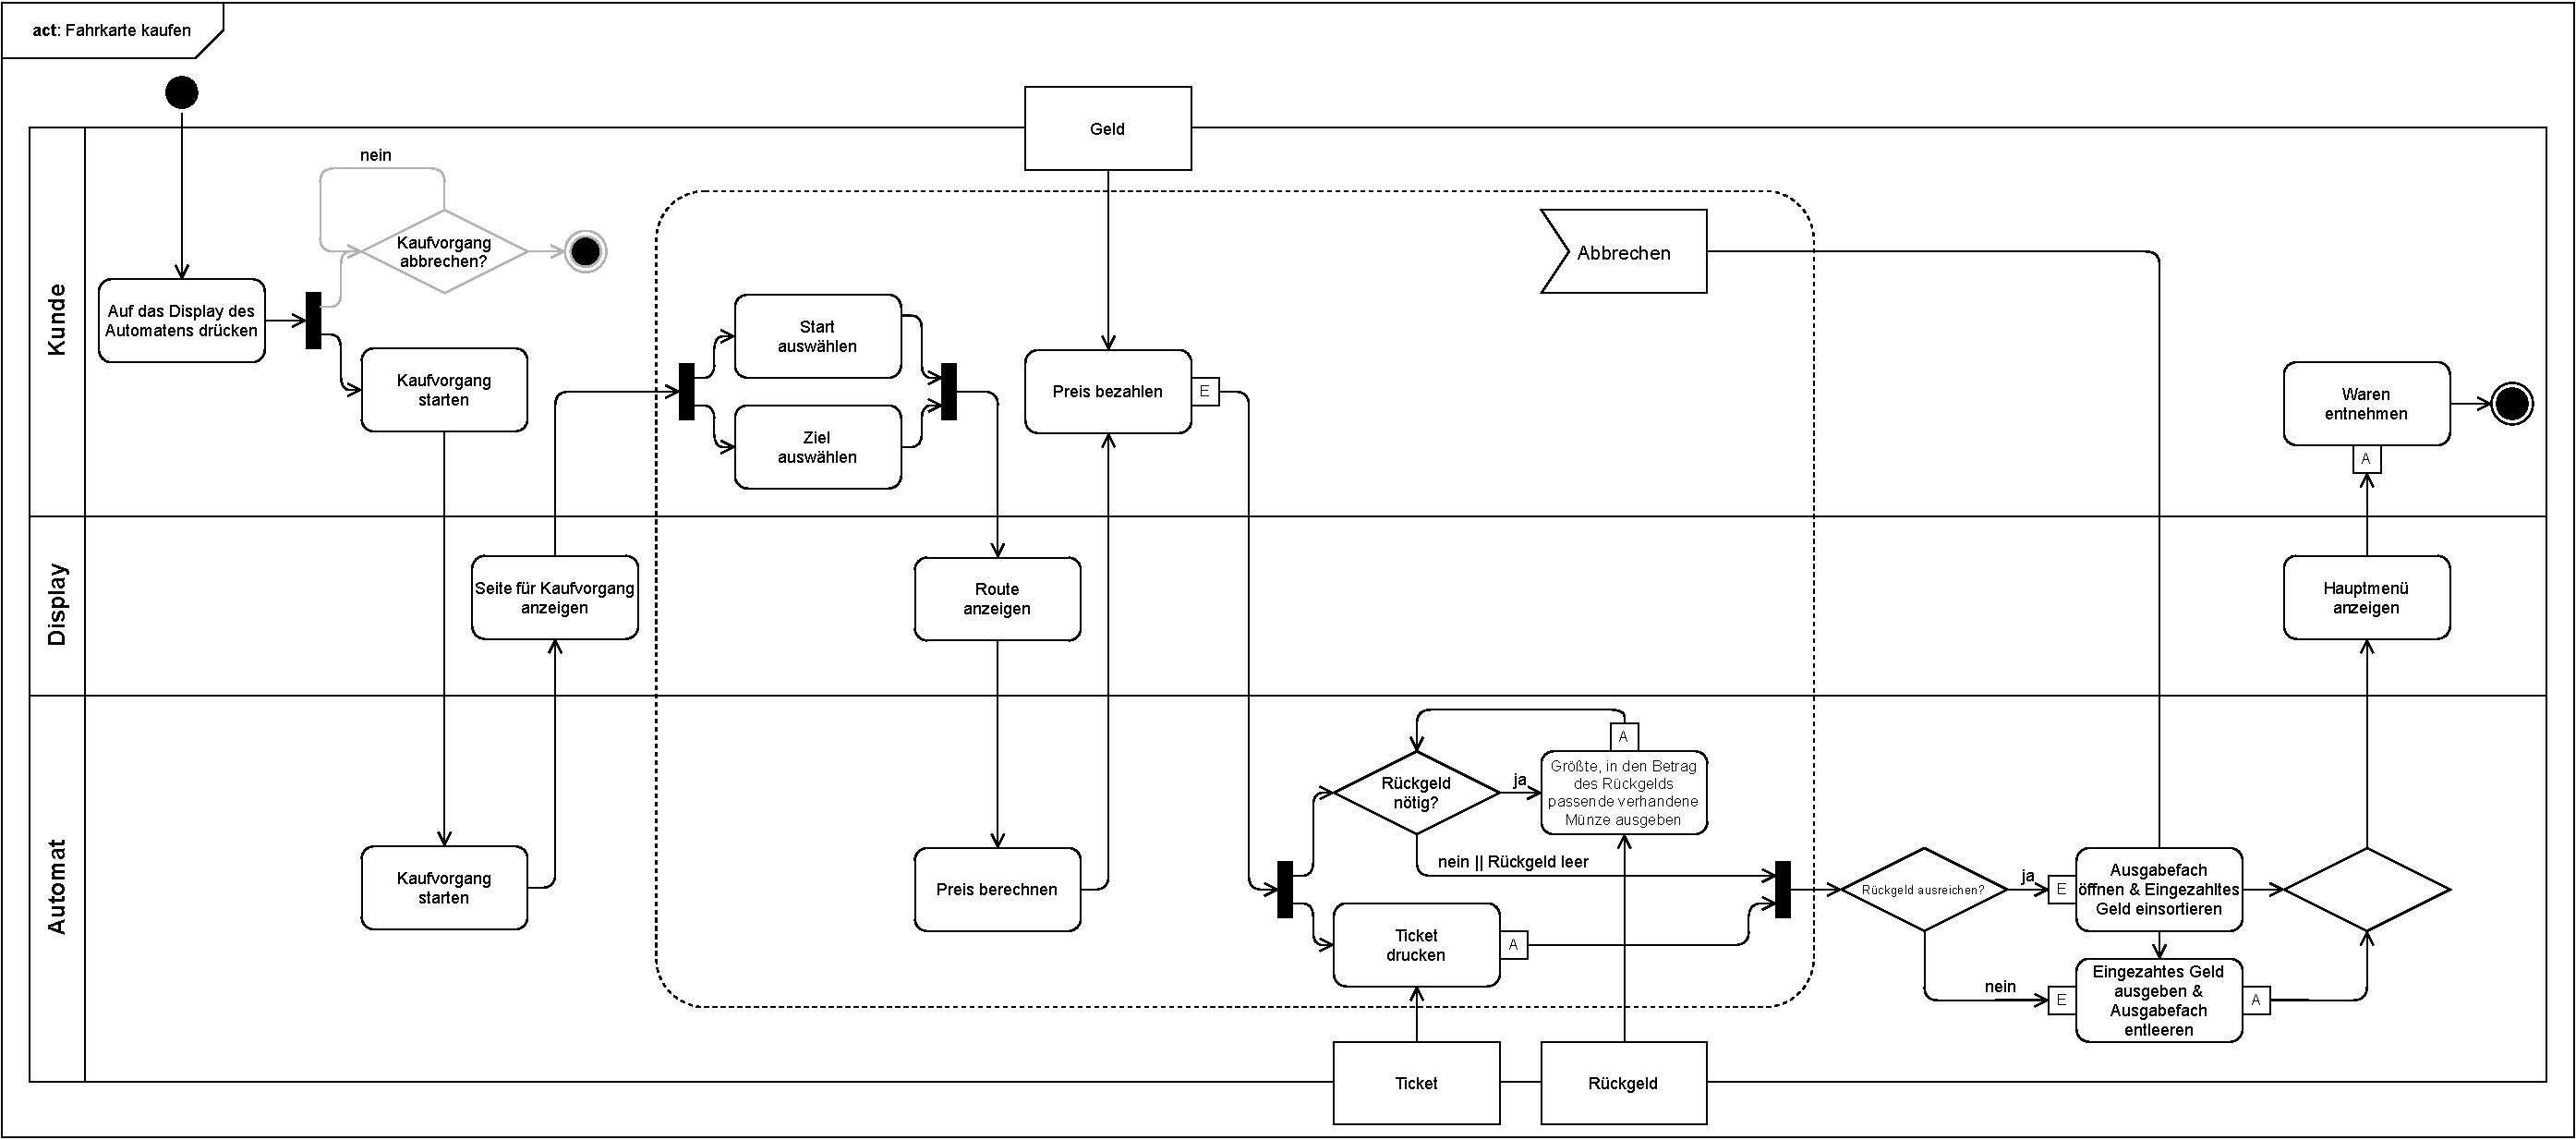
\includegraphics[width=\textwidth]{swt_wende_tim_h04_activity_diagram.pdf}
            Kommentare zum Diagramm:
            \begin{itemize}
                \item Die \gqq{Kaufvorgang abbrechen}-Loop in der oberen linken Ecke ist parallel möglich, jedoch ist ein Interrupt zugegebener Maße sinnvoller.
                    Allerdings war die \texttt{if}-Abfrage bereits fest in meinem Design verankert, also hier als alternative Darstellung ausgegraut angefügt.
                \item Um in dem Diagramm verschiedene \textbf{Objektknoten} gleichzeitig mitgeben zu können, habe ich den jeweiligen Paketen verschiedene Tagvs verliehen:
                    \begin{itemize}
                        \item E: stellt hier alle Eingaben des Benutzers dar
                        \item A: stellt alle Ausgaben des Automaten dar
                    \end{itemize}
                    Ich bin mir nicht sicher, ob das von UML 2.0 so vorgesehenen ist, jedoch empfand ich es als sinnvoll.
                \item Mein Automat besitzt ein eigenes Ausgabefach, welches nach Velieben geöffnet und geschlossen werden kann.
                    Somit ist es für den Automaten möglich, quasi jede Münze des Rückgelds einzeln auszugeben, und im späteren Verlauf alle wieder einzusammeln, ohne dass der Kunde etwaige entnehmen kann.
                    Da sich alle physischen Ausgaben des Automaten bis zum absolut sicheren Ende des Kaufvorgangs in diesem Fach befinden, können \gqq{Ticket drucken} und \gqq{Rückgeld ausgeben} parallel ablaufen.
                \item Um jedoch keine unnötigen Tickets zu drucken, ist es in meinem Automaten nicht möglich, dass die Münzen leer werden.
                    Wie man in meiner Abgabe zu Woche 3 erkennen kann, wird bei niedrigem Füllstand der Münzen ein Event ausgelöst, sodass ein Mitarbeitender der Administration diesen auffüllen kann.
                    Dies ist zwar ökologisch, jedoch nicht realitätsnah (aber hey, wir sind ja auch in SWT; ist also normal).
                \item Entschuldigung für die kleine Schrift, jedoch handelt es sich um eine \texttt{.pdf}-Datei.
                    Fühlen Sie sich frei nach Belieben reinzuzoomen.
            \end{itemize}

        \newpage
        \item Beschreiben Sie mit eigenen Worten, wie der Zusammenhang zwischen UML-Use-Case-Diagrammen, speziell der Szenariobeschreibung, und den UML-Aktivitätsdiagrammen ist.

            \begin{displayquote}
                Ein UML-Aktivitätsdiagramm beschreibt einen Pfad des Anwendungsfalldiagramms.
                Somit wird sich aus der Sicht eines beliebigen Stakeholders ein Anwendungsfall angeschaut und bis zum jeweiligen Ende weitergeführt.
                Wenn man sich die Szenariobeschreibung genauer anschaut, kann man mit cleverem kombinieren des typischen sowie aller alternativen Abläufe ein Aktivitätsdiagramm erstellen.
                So spiegeln sich alle Möglichen Ausgangszustände sowohl im Anwendungsfalldiagramm als auch im Aktivitätsdiagramm wider.
                Des Weiteren findet man die benötigten Stakeholder in den Partitionen und Ein- sowie Ausgabe als \textbf{Objektknoten} wieder.

                \vspace{1em}
                Schaut man sich beispielsweise den Anwendungsfall \gqq{Fahrkarte kaufen} an, sieht man im Aktivitätsdiagramm relativ schnell den typischen Ablauf:
                
                \vspace{1em}
                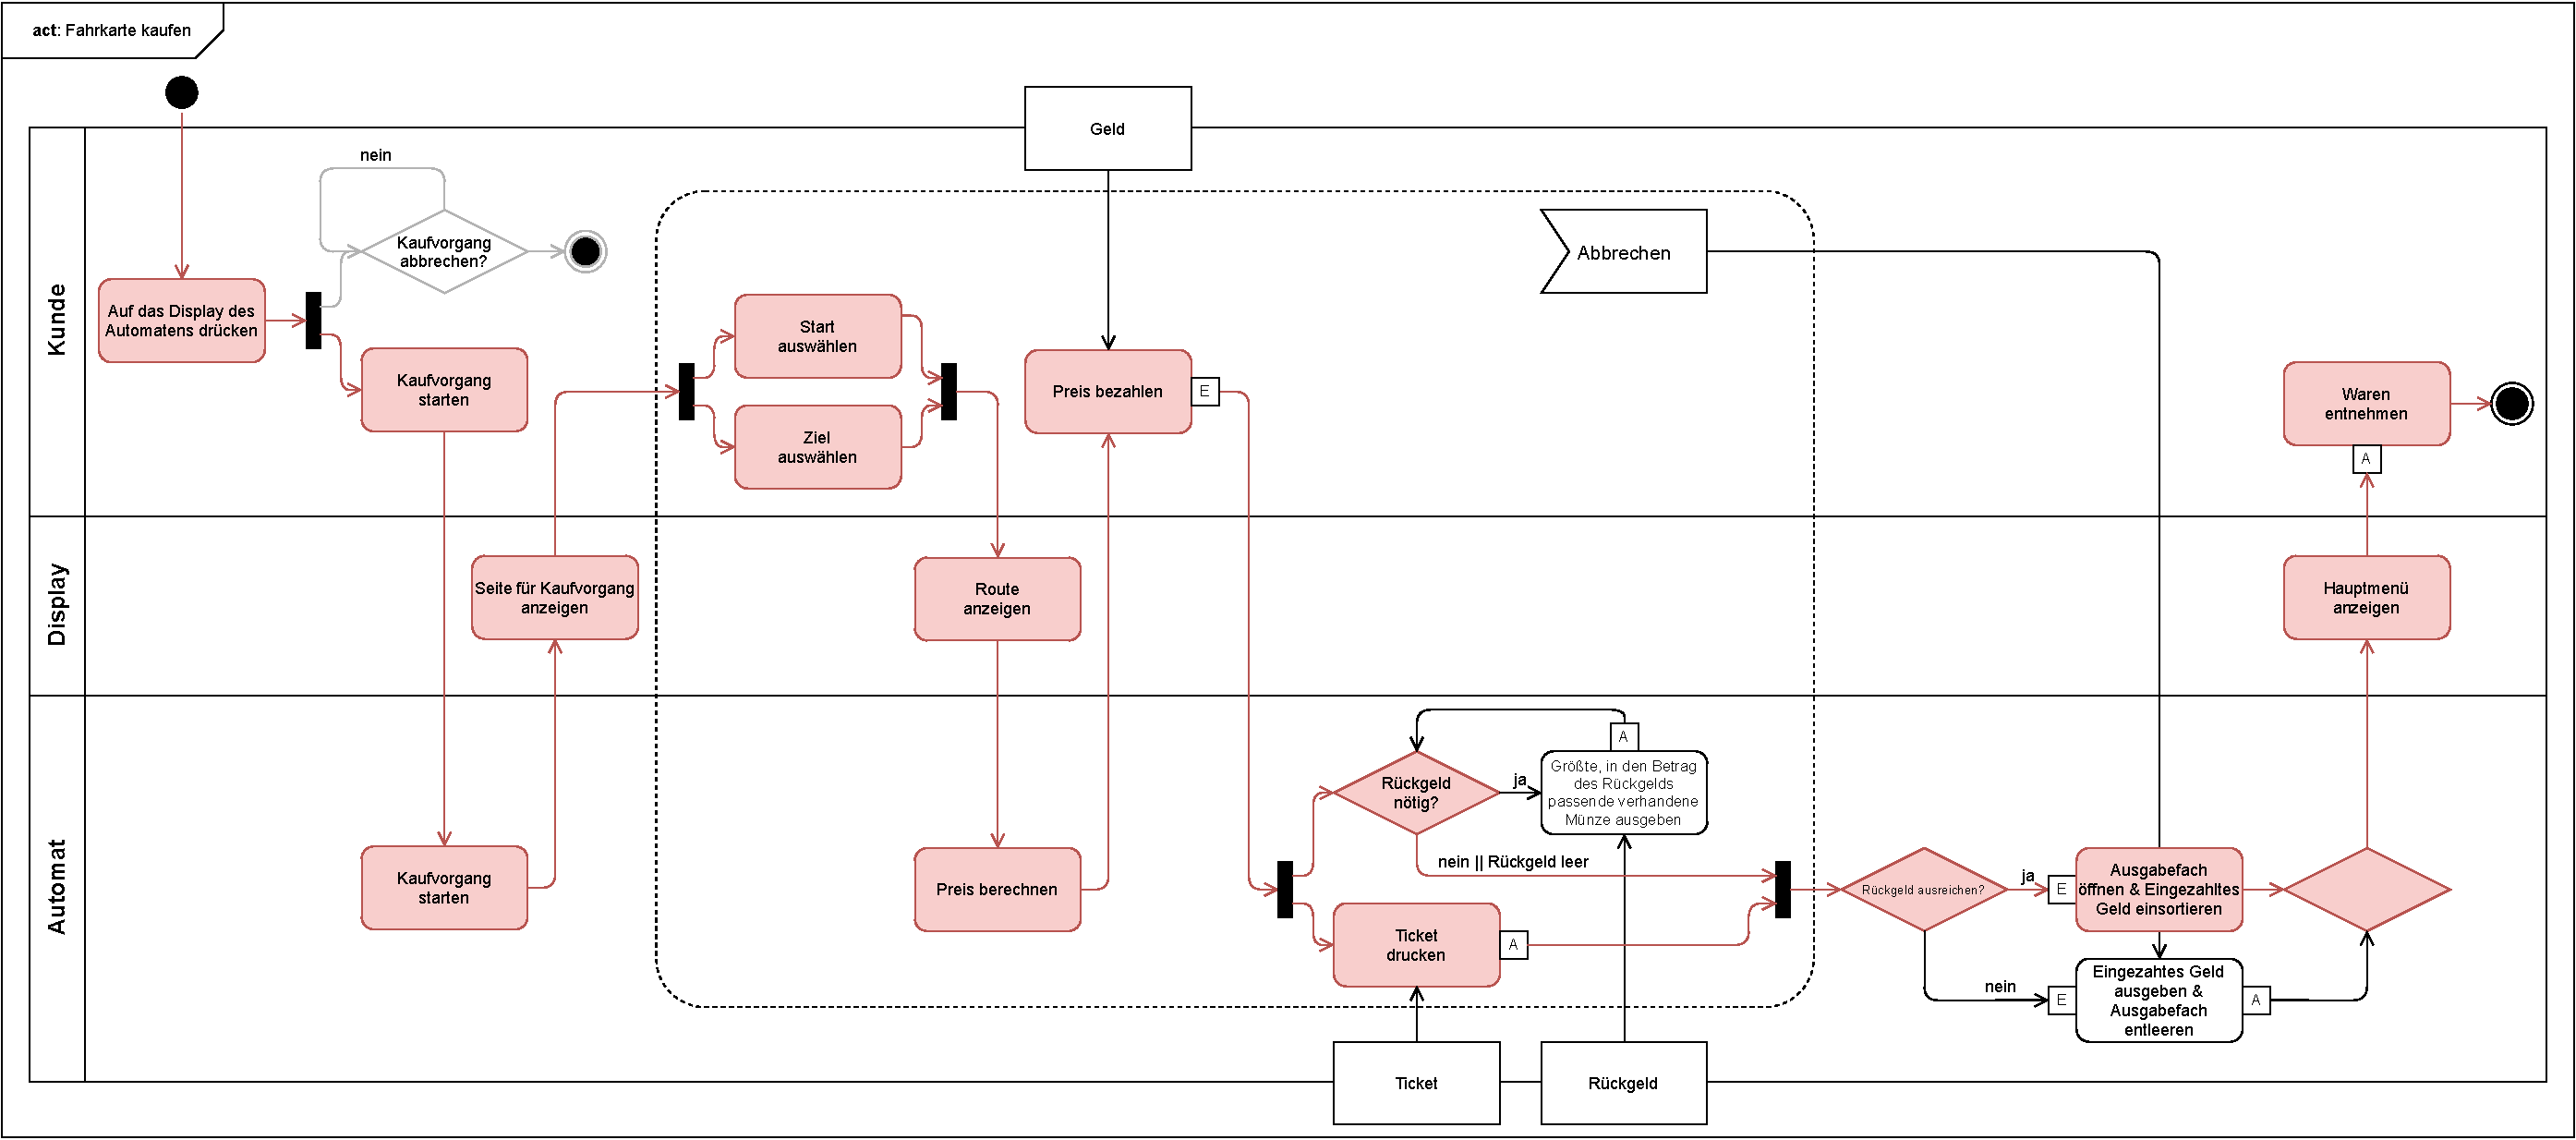
\includegraphics[width=0.95\textwidth]{swt_wende_tim_h04_activity_diagram_typical.pdf}
                \vspace{1em}

                Alternativ habe ich hier mal einen abzubrechenden Ablauf dargestellt.
                Der abbruch-Zeitpunkt ist offensichtlich variabel, ließe sich also innerhalb der \textbf{interruptable region} beliebig verschieben

                \vspace{1em}
                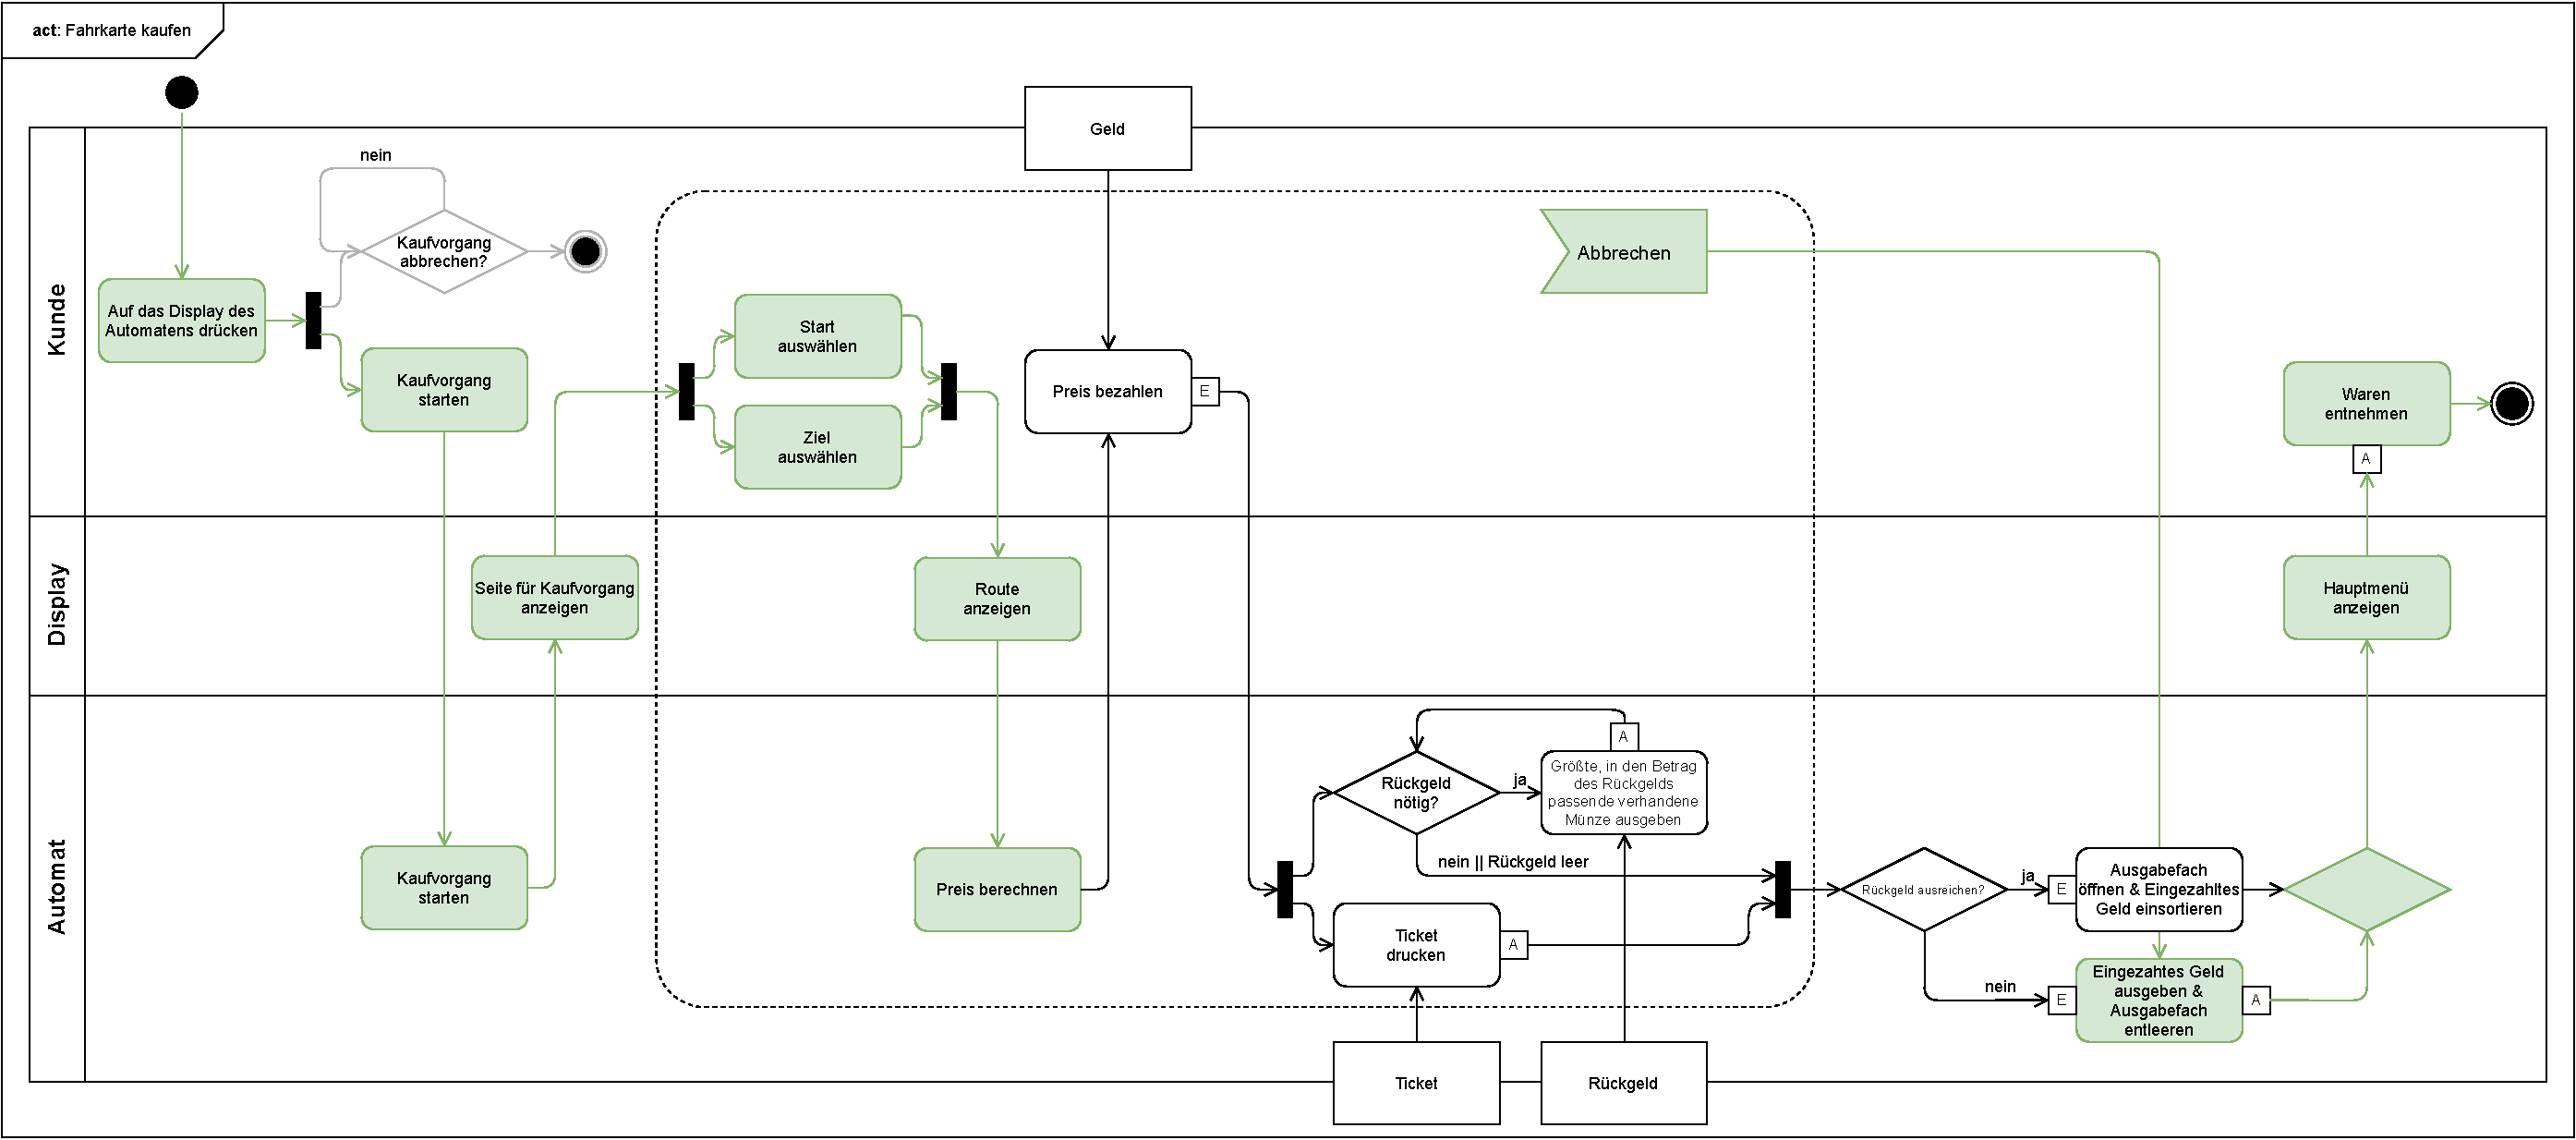
\includegraphics[width=0.95\textwidth]{swt_wende_tim_h04_activity_diagram_abort.pdf}
            \end{displayquote}

    \end{enumerate}
    
    \newpage
    \section{Klassendiagramm \& Objektdiagramm}

\end{document}